%FIGURE IMPROVEMENTS- Steering force, Drone flocking


\section{Guidance methods}
In this simulation, drones will be controlled using a combination of boid flocking behaviour\cite{boid1} and artificial potential field functions\cite{con1}.

\subsection{Potential field functions}
In a similar fashion to conservative forces such as gravity and electrostatic force, the guiding force acting on each drone can be represented as a potential field function \textbf{\(U\)}. An important property of conservative forces is:

\begin{equation}
    \vec{F} = -\Delta U = -\begin{bmatrix}\pdv{U}{x} & \pdv{U}{y}\end{bmatrix}^T
    \label{equ:force}
\end{equation}
\\
We can define the attractive potential \(U_a\) of a point as:

\begin{equation}
    U_a=\frac{1}{2}K_a\rho_a^2
    \label{equ:AtP}
\end{equation}
\noindent
       Where, \(\rho_a = \sqrt{(x - x_a)^2 + (y - y_a)^2}\) is the distance to that point and \(K_a\) is the attractive constant. This is depicted in figure \ref{fig:Atractivepot} where \(x_a\) and \(y_a\) are the coordinates of the destination and \(x\) and \(y\) are coordinates of the drone. This will be used as the guiding force towards individual destinations. Using equations \ref{equ:force} and \ref{equ:AtP} the attractive force can be found as:
       \[\vec{F_a}=\nabla U_a = \nabla \left(\frac{1}{2}K_a\Big[(x - x_a)^2 + (y - y_a)^2\Big]\right)\]
       so,
       \begin{equation} \label{equ:AtractiveForce}
       \begin{split}
                &  F_{ax} = K_a(x_a - x) \\
                &  F_{ay} = K_a(y_a - y)
        \end{split}
       \end{equation}
       which can be represented as:
       \begin{equation}
           \vec{F}_a = K_a\vert\vec{p}_{a} - \vec{p}_{d}\vert
       \end{equation}
       \noindent
       Where $\vec{p_{a}}$ and $\vec{p_{d}}$ are the attractive and drone position vectors respectively. For later simplification $|\vec{p_{a}} - \vec{p_{d}}| = \vec{V}_E$. Where $\vec{V}_E$ is the desired velocity vector in the direction of the potential field.
       \begin{figure}[h]
    \centering
    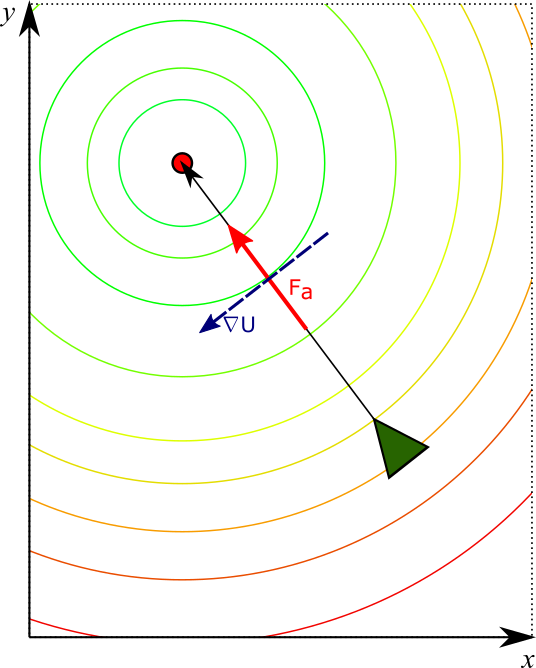
\includegraphics[width=0.25\textwidth]{figures/AtractiveForce.png}
    \caption{Potential field of destination of one drone}
    \label{fig:Atractivepot}
\end{figure}

\noindent
From figure \ref{fig:Atractivepot} it can be seen that the attractive potential is such that the force always acts towards the destination.
\clearpage

\subsection{Steering Force}

\begin{wrapfigure}{r}{0.3\textwidth}
    \begin{center}
    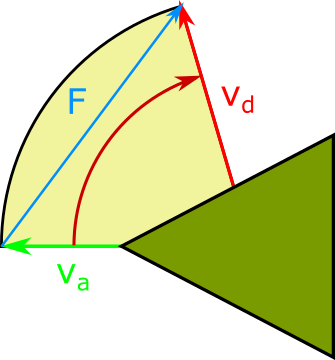
\includegraphics[width=0.2\textwidth]{figures/PropNav.png}
    \end{center}
    \caption{Steering force}
    \label{fig:PropNAv}
\end{wrapfigure}

Steering force is what gives autonomous agents the ability to steer via their own coordinate system. This simple guidance law established by Craig Reynolds \cite{boid4} is the difference between the actual velocity \(\vec{v_a}\) of the drone and the desired velocity heading \(\vec{v_d}\) determined by the behavioural model. So the steering force is:

\begin{equation}
    \vec{F} = K(\vec{v_a} - \vec{v_d})
\end{equation}

Where K is a gain which determines the weight of a specific behaviour.

\subsection{Flocking behaviour} \label{flock}
The flocking behaviour that will be introduced is from Craig Reynold's work on boids \cite{boid1} and model formulae are established from derivative work  \cite{boid3}. This uses boid steering behaviour to mimic the aggregate motion of group herding/flocking dynamics. This motion that we recognise as flocking depends upon a localised perception of the world as in nature where, in large flocks or herds, individuals are only aware of proximal members.
The local flock is determined by the perception radius, $r_p$, of each individual. Flockmates will be used to refer to  drones within the perception radius of each subject drone as demonstrated in figure \ref{fig:Flocking}. 

\begin{figure}[h]
    \centering
    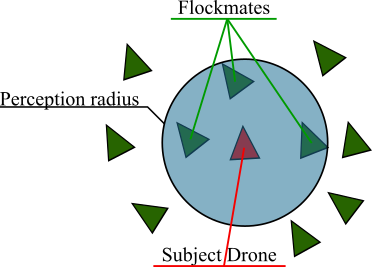
\includegraphics[width=0.5\textwidth]{figures/Flocking.png}
    \vspace{0.2cm}
    \caption{Drone flocking}
    \label{fig:Flocking}
\end{figure}

The direction and speed of every subject drone \(A\) at position \(\vec{p}_{A}\) depends on the direction and speed of all flock-mates within its perception radius \(r_p\). So for all other drones in with a position \(\vec{p_X}\) if:

\begin{equation}
    \Vert\vec{p}_{X}-\vec{p}_{A}\Vert\leq r_{p}
    \label{equ:per}
\end{equation}



\noindent


Then the drone is a flock-mate and therefore is a member of the set ${\cal{F}}_i \subset\{1,2,...N\}/\{i\}$. Otherwise, it is ignored. ${\cal{F}}_i$ then represents the set of all drones that agent $i$ is aware of.\hfill\\
\clearpage
\noindent
The localised flocking will be comprised of 3 steering behaviours that describe how the drone moves based on the velocities and positions of flock-mates. Note that || denotes a scalar vector magnitude and | is a directional vector. The behaviours are as follows:

\subsubsection{Separation}
The entity must keep its distance from other drones to avoid collisions. To achieve this the drone manoeuvres away from other drones with a force inversely proportional to the distance between them:

\begin{equation}
\vcenter{\hbox{\begin{minipage}{5cm}
\centering
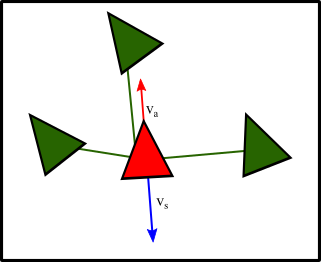
\includegraphics[width=4.5cm]{figures/Separation.png}
\captionof{figure}{Separation force}
\end{minipage}}}
\qquad\qquad
\begin{aligned}
\vec{v}_{s_i}=\sum\limits_{j={\cal{F}}_i}{\vert \vec{p}_{j}-\vec{p}_{i}\vert \over \Vert\vec{p}_{j}-\vec{p}_{i}\Vert }\\ 
so,\hspace{0.2cm}\vec{F_S}_i = K_s\vec{V}_{DS} = K_s(\vec{v}_{a_i} - \vec{v}_{s_i}) 
\end{aligned}
\label{equ:sep}
\end{equation}


\subsubsection{Alignment}
By taking the average of all velocity vectors of its flock-mates, each drone steers into alignment with its flock-mates. The flock comes to a consensus of heading through velocity matching.\hfill

\begin{equation}
\vcenter{\hbox{\begin{minipage}{5cm}
\centering
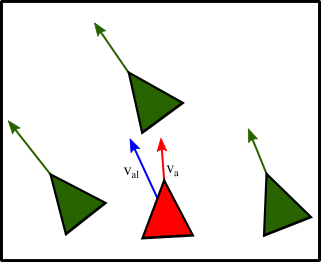
\includegraphics[width=4.5cm]{figures/Alingment.png}
\captionof{figure}{Alignment force}
\end{minipage}}}
\qquad\qquad
\begin{aligned}
\vec{v}_{al_i}=\sum\limits_{j={\cal{F}}_i}\vec{v_j}\\
so,\hspace{0.2cm}\vec{F_{Al_i}} = K_{al}\vec{V}_{DA} = K_{al}(\vec{v}_{a_i} - \vec{v}_{al_i})
\end{aligned}
\label{equ:al}
\end{equation}


\subsubsection{Cohesion}
This is what keeps the flock grouped together. Members of the flock move towards the average position of the flock. This includes the subject drone position.

\begin{equation}
\centering
\vcenter{\hbox{\begin{minipage}{5cm}

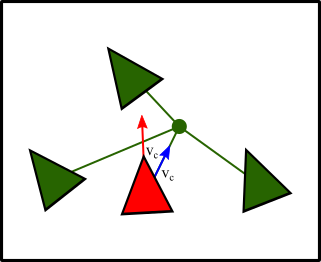
\includegraphics[width=4.5cm]{figures/Cohesion.png}
\captionof{figure}{Cohesion force}
\end{minipage}}}
\qquad\qquad
\begin{aligned}
\vec{v}_{c_i}= {\vec{p}_{i} + {{\sum\limits_{j={\cal{F}}_i}\vec{p}_{j}}}}\\ 
so,\hspace{0.2cm}\vec{F_{C_i}} = K_c\vec{V}_{DC}= K_c(\vec{v}_{a_i} - \vec{v}_{c_i})
\end{aligned}
\label{equ:coh}
\end{equation}

\noindent
\(K_s\), \(K_{al}\) and \(K_c\) are the separation gain alignment gain and cohesion gain respectively. They drive the flocking behaviour of the agent by increasing the magnitude of velocity vectors $\vec{V}_{DS}$, ${al}\vec{V}_{DA}$ and $\vec{V}_{DC}$.
\clearpage

